\documentclass[10pt]{article}

\usepackage[T1]{fontenc}
\usepackage[utf8]{inputenc}
\usepackage[english]{babel}
\usepackage{multicol}
\usepackage{graphicx}
\usepackage{lmodern}
\usepackage{amsmath}
\usepackage{amsthm}
\usepackage{cases}
\usepackage{amssymb}
\usepackage{amsfonts}
\usepackage{pdfpages}
\usepackage[margin=60pt]{geometry}
\usepackage{abstract}
\renewcommand{\abstractnamefont}{\normalfont\Large\bfseries}
\renewcommand{\abstracttextfont}{\normalfont\normalsize}

\usepackage{float}
\floatstyle{boxed}
\newfloat{boxframe}{H}{}
\floatname{boxframe}{Box}

\newcommand{\ud}{{\mathrm{d}}}
\newcommand{\pr}{{\mathbb{P}}}
\newcommand{\nN}{{n_\textrm{H}}}
\newcommand{\nI}{{n_\textrm{I}}}
\newcommand{\Xnema}{\textit{X. nematophila} }
\newcommand{\Scarpo}{\textit{S. carpocapsae} }
\newcommand{\XNema}{\textit{Xenorhabdus nematophila} }
\newcommand{\SCarpo}{\textit{Steinernema carpocapsae} }
\newcommand{\IBD}{IBD}
\newcommand{\qw}{Q_\mathrm{w}}
\newcommand{\qb}{Q_\mathrm{b}}

\author{Latrille Thibault\\
\small thibault.latrille@ens-lyon.fr\\[-0.8ex]}
\title{Model of cooperative strategies, the case of nematode-borne insect
pathogen \Xnema} 
\begin{document}
%\includepdf[pages={1}]{first_page.pdf}
\begin{abstract}
The bacterium \Xnema inhabits and influences the lives of two host animals, helping one to reproduce optimally while killing the other. Many studies focused on the symbiotic association between bacteria and hosts, but they scarcely focused on cooperation at the bacterial level. We here provide evidence that the parasitic life cycle of these bacteria has a lot of influence on their relatedness, and thus on cooperation between bacteria. Cooperative evolutionary strategies of bacteria are investigated in the light of their symbiotic life cycle. We here provide ground on the occurrence that the critical phase driving evolutionary strategies is the infection by nematodes. Yet this phase had not been extensively investigated experimentally. We provide a null model that predict experimental results. 
mutualistic / pathogenic 

\smallskip
\noindent \textbf{Keywords.} symbioses, cooperation, 
\end{abstract}
\begin{multicols}{2}
\section*{Introduction}
The $\gamma$-proteobacterium \XNema colonizes the entomopathogenic nematode \SCarpo in a mutualistic association, and is also a pathogen of insects. 
The mutualistic relationship between \Xnema and \Scarpo is not obligate, as both partners can survive in the absence of the other; however, \Xnema is required for \Scarpo nematodes to reproduce efficiently during their lifecycle. 
\Scarpo nematodes are either found in insect hosts or in the soil. The soil-dwelling vector stage, called the infective juvenile (IJ), is encased in a double cuticle, and is non-feeding owing to its closed mouth and anus.
Prior to the IJ stage, ingested \Xnema bacteria colonize \Scarpo at a discrete intestinal location known as the vesicle. 
The IJ nematode then serves as a vector, carrying \Xnema into a susceptible insect, in which it is released from its nematode vector and rapidly kills the insect. 
\Xnema is capable of killing insects in the absence of \Scarpo by direct injection of \Xnema cells in the laboratory. 
\Xnema is capable of long-term survival in any reservoir outside its animal hosts in nature and, therefore, may rely on its nematode vector for transmission. 
The insect carcass provides nutrients for the propagation of both nematode and bacterium. 
In response to a signal, possibly nutrient deprivation or space limitation, \Xnema re-associates with the nematode, and the pair leave in search of a new insect host to repeat the cycle.
\Scarpo nematodes are easily propagated; several hundred thousand IJs can be generated from the infection of a single insect host or from lawns of X. nematophila and can be stored in water or buffer for weeks. 
Unlike many animals associated with bacterial mutualists, \Scarpo nematodes are viable in the absence of \Xnema Therefore, aposymbiotic nematodes can be obtained and assessed for responses to diverse bacterial and environmental stimuli. 
Haemolymph supports vigorous growth of X. nematophila (0.41 doublings per hour in haemolymph) even during release from the nematode. By contrast, the maximum \Xnema growth rate observed in the nematode vesicle was 0.1 doublings per hour, indicating that this environment is comparatively nutrient limiting.
The \Xnema population within an IJ nematode is founded by between one and two individual bacterial cells that grow to fill the vesicle, which is the lumen between two nematode epithelial cells at the anterior end of the intestine\cite{Martens}. The specificity is very stringent since other Xenorhabdus species do not colonize \Scarpo IJs.

Although \Xnema model is emerging as an invaluable tool for elucidating microorganism–host interactions. Many studies solely focused on the symbiotic association between the $\gamma$-protecterium and its hosts, but the scarcely discussed the cooperation at the bacterial level. We here provide evidence that the parasitic life cycle of these bacteria has a lot of influence on their relatedness. Thus evolutionary strategies of bacteria are investigated in the light of their symbiotic life cycle.

Relatedness is a key component of inclusive fitness, it is a measure of how closely two individuals are related. The relatedness is highly dependent on the genealogy of the population and of recent coalescent, thus population dynamic is closely related to relatedness. We here derived formulas for relatedness under several models of stochastic population dynamic. Deterministic approximation are made subsequently when calculus taking into account stochasticity become intractable. Our models seek to describe the biological case of a bacteria, the nematode-borne insect pathogen \Xnema.

The first section is dedicated to derive evolutionary strategies of bacteria as a function of relatedness. Subsequent section are devoted to derive the formula of the relatedness under two  model of infections of the insect by the nematodes. The former is considering all nematodes infect the insect simultaneously as propagules. The latter assume the nematodes arrive successively.
\begin{figure*}[ht]
	  \centering
	  \label{fig:life_cycle}
       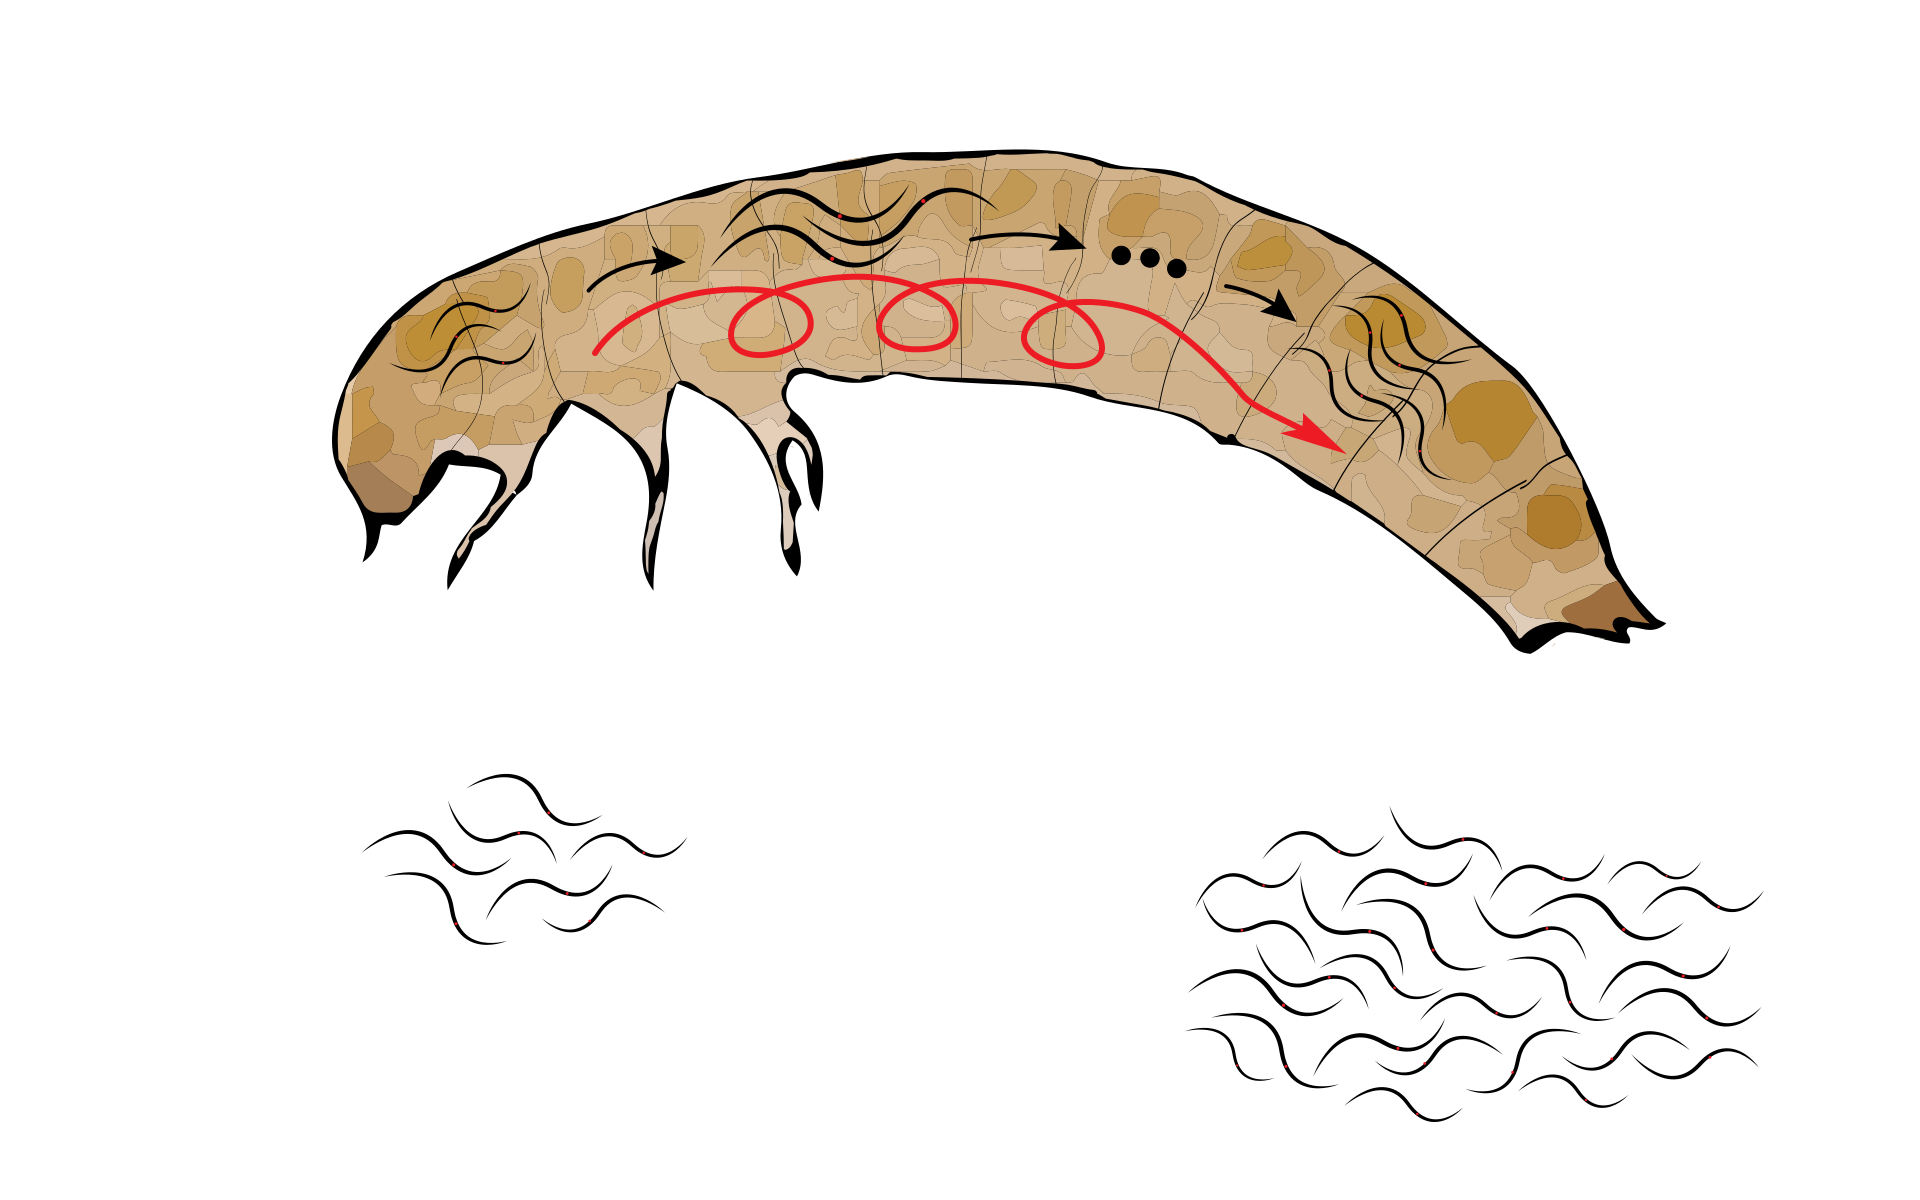
\includegraphics[width=10.0cm]{Figures/Life_cycle.png}\\
		\caption{ \textbf{The life cycle.}
		}
\end{figure*}
\section*{Fitness function and derivation of equilibrium.}
Experimentally, \Xnema is found  in the insect in two types I and II (references).
Isogenic bacteria. There exist evidence that a molecular switch can make that possible. Meaning type I switch to type II, and this is irreversible. Type II die off but increase the number of nematodes that make it to the next cycle. Various biological scenario are expected to produce such effect. For example bacteria can produce bactericides or fungicides that kill-off unwanted guests, thus increasing the foraging of the host by the nematodes. Or they can sacrifice themselves to nourish the nematode.
There is a trade off, by switching to type II, a bacterium drastically reduce its own fitness but increases the fitness of neighbors, thus increasing its inclusive fitness.
We seek to reflect this phenomenon in our model, where the phenotype under investigation is $z$, the probability that a focal bacterium switch to type II.
We assume this phenotype is only expressed after the exponential growth of bacteria. 
We assume the fitness of nematodes is an increasing linear mapping of the phenotype under investigation: $f (z)=az+b$, $a<0$.
By denoting $z_\bullet $ the phenotype $z$ for the focal bacterium, $ z_0^{\mathrm{R}}$ the average phenotype $\bar{z}$ for the individuals in the same deme as the focal individual and 
  Under the model of infinite number of demes (insects), the fitness of the focal bacterium is:
  \begin{equation}
  w(z_\bullet ,z_0^{\mathrm{R}} , \bar{z} ) = \dfrac{1-z_\bullet}{1- z_0^{\mathrm{R}}}\dfrac{a z_0^{\mathrm{R}} +b }{a \bar{z} +b}.
  \end{equation}
  We then compute the partial derivative of the fitness with regard to $z_\bullet$ and $z_0^{\mathrm{R}}$ and evaluate them at $z$:
  \begin{equation}
   \left. \dfrac{\partial w(z_\bullet ,z_0^{\mathrm{R}} , \bar{z} )}{\partial z_\bullet} \right\vert_{z_\bullet = z_0^{\mathrm{R}} = \bar{z}=z} = \dfrac{1}{ z-1 }.
  \end{equation}
  \begin{equation}
   \left. \dfrac{\partial w(z_\bullet ,z_0^{\mathrm{R}} , \bar{z} )}{\partial z_0^{\mathrm{R}}} \right\vert_{z_\bullet = z_0^{\mathrm{R}} = \bar{z}=z} = \dfrac{a +b}{( z - 1 )(a z +b)}.
  \end{equation}
  Solving $\left. \dfrac{\partial w}{\partial z_\bullet} \right\vert_{z^*} + \left. \dfrac{\partial w}{\partial z_0^{\mathrm{R}}} \right\vert_{z^*} R =0 $ yields a candidate evolutionary stable strategy, see \cite{rousset2004genetic}.
    \begin{equation}
  \dfrac{1}{ 1 - z^* } + \dfrac{a +b}{(1- z^*)(a z^* +b)}R =0
  \end{equation}
  \begin{equation}
  \iff
  \end{equation}
  \begin{equation}
  z^*=\dfrac{R(a+b)-b}{a}=R(1+c)-c \text{ where }c=\dfrac{b}{a}.
  \end{equation}
  In the special case $c=0$, meaning there is no threshold, the phenotype is equal to the relatedness:
  \begin{equation}
  z^*=R.
  \end{equation} 
  It is worth noting that if $R<\dfrac{c}{c+1}$, then the candidate evolutionary stable strategy is no cooperation $(z^*=0)$.
\section*{Model of infections}
\subsection*{Consecutive infections.}
Taking mutation rate $u$ into account, in a similar fashion to \cite{rousset2004genetic}, the recursion equations are: 
  \begin{subnumcases}{\hspace*{-0.7cm}}
      		\qw ' = (1-u)^2 \left[ \psi + \left( \dfrac{ \qw }{\nI}+\dfrac{\nI-1}{\nI} \qb \right) (1 -\psi) \right] \\
    		\qb ' = (1-u)^2 \left[ \dfrac{ \qw }{\nI}+\dfrac{\nI-1}{\nI} \qb \right].
  \end{subnumcases}
 At equilibrium, $\qw ' = \qw$ and $\qb ' =\qb$ and the recursion equations are:
  \begin{subnumcases}{\hspace*{-0.7cm}}
      		\qw = (1-u)^2 \left[ \psi + \left( \dfrac{\qw}{\nI}+\dfrac{\nI-1}{\nI} \qb \right) (1 -\psi) \right] \\
    		\qb = (1-u)^2 \left[ \dfrac{\qw}{\nI}+\dfrac{\nI-1}{\nI} \qb \right].
  \end{subnumcases}
 Leading to the unique solution:
   \begin{subnumcases}{\hspace*{-0.7cm}}
 \qw = \dfrac{ (1-u)^2 [u (2 - u)(\nI-1) +1 ]\psi }{ u (2-u )(\nI - \psi )+\psi }\\
 \qb = \dfrac{(1- u )^4 \psi}{u (2-u) (\nI - \psi ) +\psi}.
  \end{subnumcases}
 And the relatedness is: 
 \begin{align}
 R &= \dfrac{\qw - \qb }{1- \qb} \\
   &=\dfrac{(1-u)^2 \nI \psi}{\nI +(1-u)^2 \psi}.
 \end{align}
And thus by taking the limit for low mutation rate ($u \rightarrow 0$), the relatedness becomes:
 \begin{equation}
 R \simeq \dfrac{\psi}{1+ \dfrac{\psi}{\nI}}.
 \end{equation} 
Under the assumption of an important number of demes ($\nI \rightarrow \infty$), the relatedness is:
 \begin{equation}
 R \simeq \psi 
 \end{equation}
 It is worth noting that the relatedness does not depend on the number of bacteria initially brought by the nematode ($r$), nor on the the total population size when the bacteria stop growing exponentially. 
 This formula is valid only if the population of bacteria is growing exponentially at the time the last nematode infected the insect.

\subsection*{Simultaneous infections by propagules.}

The life cycle of the bacteria involve two hosts, nematodes and insects. The nematode is considered as the vector of the bacteria they carry around a hundred of them, and both are needed to infect the insect.
Let $Q_i$ be the probability of identity of genes from different bacteria, within the same insect ($\qw$) and in different insect ($\qb$). Here we consider the probability of identity 
in the infinite allele model, and let $u$ be the mutation rate.
 The recursion equations for next generation identities $\qw '$ and $\qb '$ are: 
  \begin{subnumcases}{\hspace*{-0.8cm}}
      		 \qw ' = (1-u)^2[\psi + (1 -\psi) ( \phi \qw + (1-\phi) \qb ]  \\
    		 \qb ' = (1-u)^2 \left[ \dfrac{ \qw }{\nI}+\dfrac{\nI-1}{\nI} \qb \right].
  \end{subnumcases}
  At equilibrium, $\qw ' = qw$ and $\qb ' =\qb$ and the recursion equations are:
  \begin{subnumcases}{\hspace*{-0.8cm}}
      		 \qw = (1-u)^2[\psi + (1 -\psi) ( \phi \qw + (1-\phi) \qb ] \\
    		 \qb = (1-u)^2 \left[ \dfrac{ \qw }{\nI}+\dfrac{\nI-1}{\nI} \qb \right].
  \end{subnumcases}
  This simultaneous can be solved unambiguously and leads to the relatedness
  \begin{align}
 R &= \dfrac{\qw - \qb }{ 1- \qb } \\
 &= \dfrac{ \psi (1-u)^2 }{ 1 - (1-u)^2 \phi (1- \psi )+(1-u)^2 / \nI } .
 \end{align}
And thus by taking the limit for low mutation rate ($u \rightarrow 0$), the relatedness becomes:
 \begin{equation}
 R \simeq \dfrac{ \psi  }{ 1 - \phi (1- \psi )+1 / \nI }.
 \end{equation} 
Under the assumption of an important number of demes ($\nI \rightarrow \infty$), the relatedness $R$ is:
 \begin{equation}
 R \simeq \dfrac{ \psi  }{ 1 - \phi (1- \psi ) }
 \end{equation}

\section*{Probability of identity}

\subsection*{Synchronous infections}
Biologically, these assumption reflect the fact that we neglect competition, and also that the probability for a bacteria to divide is independent of its age.
The model is the following, $d$ nematodes infect an insect simultaneously (at time $t=0$). The probability of identity $\psi(t)$ is:
\begin{align}
\psi(t) &= \dfrac{ r_+ + \sum_{i=1}^d r_i^2}{r_+ (r_+ +1)}  -2 e^{-\lambda t} \dfrac{ r_+^2-\sum_{i=1}^d r_i^2}{r_+ (r_+^2 -1) }. \label{psi_simultaneous} 
\end{align}
Under the assumption $r_i \gg 1$, $ 1 \leq i \leq d $, the approximation of $\psi(t)$ becomes independent of $t$:
 \begin{equation}
\psi \simeq \displaystyle \sum_{i=1}^d \left( \dfrac{ r_i}{\sum_{i=1}^d r_i} \right)^2.
 \end{equation}
We also assume that each nematode carry the same number of bacteria. Mathematically, that is to say the $r_i$ are constant and equal $r$ for $0 \leq i \leq d$. The probability of identity $\psi$ reduces to:
\begin{equation}
\psi = \dfrac{1}{d}
\end{equation}
 This approximation is of particular interest. Indeed, providing the number of initial individual is large enough ($r_i \geq 100$), the probability of identity does not change over time and depends solely on the initial number of the nematodes. 

\end{multicols}
\begin{boxframe}
\label{box_PI_simultaneous}
\begin{multicols}{2}
\textbf{Box 1. Proof of the formula \eqref{psi_simultaneous}}
The insect is infected by $d$ nematodes at time $t=0$. Each nematode $i$ ($ 1 \leq i \ d$) releases $r_i$ bacteria inside the insect. We assume the $d$ independent lineages immediately enter the growth process. The growth process described is a Markov process. We assume that each bacteria has an independent constant birth rate $\lambda$ and that they never die. The Kolmogorov forward equations describing the population size $N_i(t)$ of the $i$th lineage is:
 $N_i(t)$ is of the negative binomial form \cite[p. 158]{cox1977theory}, and for $n \geq r_i$: 
\begin{equation}
\pr(N_i(t)=n)=\binom{n-1}{r_i-1} \left( e^{-\lambda t} \right)^{r_i} \left( 1-e^{-\lambda t} \right)^{n-r_i}.
\end{equation}
We are interested in variable 
 $ r_+=\sum_{i=0}^d r_i$ is the initial size of the population \\
 $\quad N_+(t)=\sum_{i=0}^d N_i(t)$ is the random variable denoting the size of the population at time $t$ \\
 Let us denote $X_i(t)=N_i(t)-r_i$, the number of births. $X_+(t)=N_+(t)-r_+$ is independent negative binomials is a negative binomial \cite{johnson2005univariate}:
\begin{equation}
 X_+(t)  \sim \mathrm{NB} \left( r_+, e^{-\lambda t} \right).
\end{equation}
Thus the distribution of $X_i(t)$ conditional on $ X_+(t)=x_+$ is a negative hypergeometric and is independent of $e^{-\lambda t}$:
\begin{align}
\pr( X_i & (t) =x \vert X_+(t)=x_+ )  \nonumber \\ 
& = \dfrac{\displaystyle \binom{x+r_i-1}{x} \binom{x_+-x+r_+-r_i-1}{x_+-x}}{\displaystyle \binom{x_+ +r_+ -1}{x_+}}.
\end{align}
Leading to expectation for $X_i(t)(X_i(t)-1)$ conditional on $X_+(t)$:
\begin{equation}
 \mathbb{E} [ X_i(t)(X_i(t)-1) \vert X_+(t) ] =\dfrac{r_i(r_i+1)}{r_+ (r_+ +1 )}X_+(t) ( X_+(t) -1 ).
\end{equation}
Thus we access the expectation of $N_i(t)(N_i(t)-1)$ conditional on $N_+(t)$:
\begin{align}
 \mathbb{E} & [ N_i(t) (N_i(t)-1) \vert N_+(t) ]   \nonumber \\
 &=\dfrac{r_i(r_i+1) }{r_+ (r_+ +1)}N_+(t) ( N_+(t) -1 ) -\dfrac{2 r_{i} (r_+ - r_i) }{r_+ (r_+ +1)} N_+(t)
\end{align}
Leading to the expectation of $Z_i(t)$ conditional on $N_+(t)$.
\begin{align}
  \mathbb{E} [  Z_i(t)  & \vert N_+(t) ] = \mathbb{E}\left[ \left. \dfrac{N_i(t)(N_i(t)-1)}{N_+(t)( N_+(t)-1 ) }  \right\vert N_+(t) \right] \\
 &= \dfrac{r_i(r_i+1)}{r_+ (r_+ +1)}- \dfrac{2 r_i (r_+ -r_{i})}{r_+ (r_+ +1)} \dfrac{1}{ N_+(t) -1  }.
\end{align}
And by the law of conditional expectation:
\begin{align}
\mathbb{E}\left[ Z_i(t) \right] &= 
 \mathbb{E}\left[ \mathbb{E}\left[ \left. Z_i(t) \right\vert N_+(t) \right] \right]\\
 &=\dfrac{r_i(r_i+1)}{r_+ (r_+ +1 )}-\dfrac{2 r_i (r_+ -r_{i})}{r_+ (r_+ +1 )}\mathbb{E}\left[\dfrac{1}{N_+(t)-1} \right]. 
\end{align}
Since $N_+(t) \sim \mathrm{NB} (r_+, \pi(t))$ we have:
\begin{align}
\mathbb{E}\left[\dfrac{1}{N_+(t)-1} \right]=\dfrac{e^{-\lambda t}}{r_+-1}.
\end{align}
And thus 
\begin{align}
\mathbb{E}\left[ Z_i(t) \right] =\dfrac{r_i(r_i+1)}{r_+ (r_+ +1 )}-2e^{-\lambda t}\dfrac{ r_i (r_+ -r_{i})}{r_+ (r_+^2 -1 )}.
\end{align}
By summing previous over all $i$, we evaluate the probability of identity $\psi(t)$:
\begin{align}
\psi(t) &= \mathbb{E}[\sum_{i=1}^d Z_i(t)] \\
 &=\dfrac{ r_+ + \sum_{i=1}^d r_i^2}{r_+ (r_+ +1)}  -2 e^{-\lambda t} \dfrac{ r_+^2-\sum_{i=1}^d r_i^2}{r_+ (r_+^2 -1) }.
\end{align}
 \end{multicols}
\end{boxframe}
\begin{multicols}{2}

\subsection*{Succesive infections}

  We derive the formula for two nematodes arriving at different times. We assume nematodes arrive at times exponentially distributed of parameter $ \tau$. If we assume the lineage carried by the first vector grew in a deterministic fashion, then its size is $r e^{\lambda  T}$. $\omega=\tau / \lambda$
\begin{equation}
   \psi = 1- 2 \omega \mathrm{B}_{1/2}(1+\omega,1-\omega), \label{psi_consecutive}
\end{equation}
where $\mathrm{B}_x(a,b)$ is the incomplete beta function:
\begin{align}
\mathrm{B}_x(a,b) = \int_0^x t^{a-1}(1-t)^{b-1} \ud t.
\end{align}
Calculus become intractable when there is more than two nematodes arriving in the insect. Thus we are considering nematodes arriving at constant times in the next subsection, which is a strong assumption.


\end{multicols}
\begin{boxframe}
\label{box_PI_simultaneous}
\begin{multicols}{2}
\textbf{Box 2. Proof of  the formula \eqref{psi_consecutive}}
We derive the formula for two nematodes arriving at different times. We assume nematodes arrive at times exponentially distributed of parameter $ \tau$. Let us stop the time at the moment the second (and last) nematode infected the insect, the nematode releases $r$ bacteria into the insect. The first one arrived at time $T$ before, where $T\sim \exp ( \tau)$. If we assume the lineage carried by the first vector grew in a deterministic fashion, then its size is $r e^{\lambda  T}$. \\
  The continuous random variable equal to the proportion of bacteria from the lineage carried by the first nematode is $\dfrac{r e^{\lambda T}}{r+re^{\lambda T}}=\dfrac{ e^{\lambda T}}{1+e^{\lambda T}}$. In a similar fashion, the continuous random variable equal to the proportion of bacteria from the lineage carried by the second nematode is $\dfrac{1}{1+e^{\lambda T}}$.
  \begin{align}
  \psi  &=\mathbb{E} \left[ \left( \dfrac{ e^{\lambda T}}{1+e^{\lambda T}} \right)^2+\left( \dfrac{1}{1+e^{\lambda T}} \right)^2 \right] \\
  &=\int_0^\infty \left( \left( \dfrac{ e^{\lambda t}}{1+e^{\lambda t}} \right)^2 + \left( \dfrac{1}{1+e^{\lambda t}} \right)^2 \right) \tau e^{ -\tau t } \ud t.
  \end{align}
  The evaluation of this integral is not straightforward. Instead we derive the cdf and pdf of $\dfrac{ e^{\lambda T}}{1+e^{\lambda T}}$ and $\dfrac{ e^{\lambda T}}{1+e^{\lambda T}}$.
  \begin{align}
  F_1(p) &\equiv \pr \left(\dfrac{e^{\lambda T}}{1+e^{\lambda T}} \leq p\right)= \pr \left(T \leq \lambda^{-1} \mathrm{ln}\left( \dfrac{p}{1-p} \right) \right) \\
  &= 1-(1-p)^{\omega} p^{-\omega} \text{ for } 1/2 \leq p \leq 1.
  \end{align}  
  \begin{align}
  F_2(p) &\equiv \pr \left(\dfrac{1}{1+e^{\lambda T}} \leq p\right) = \pr \left(T \geq \lambda^{-1} \mathrm{ln}\left( \dfrac{1-p}{p} \right) \right) \\
  &= (1-p)^{-\omega} p^\omega \text{ for } 0 \leq p \leq 1/2.
  \end{align}
  And we have the pdf of $P_1$ and $P_2$ is:
  \begin{align}
  f_1(p) &= \dfrac{ \ud F_1(p) }{ \ud p} =  \omega (1-p)^{\omega-1} p^{-\omega-1}  \text{ for } 1/2 \leq p \leq 1\\
  f_2(p) &= \dfrac{ \ud F_2(p) }{ \ud p} =  \omega (1-p)^{-\omega-1} p^{\omega-1} \text{ for } 0 \leq p \leq 1/2.
  \end{align}
  And 
  \begin{align}
  \psi &= \int_{1/2}^{1} p^2 f_{P_1}(p) \ud p + \int_{0}^{1/2} p^2 f_{P_2}(p) \ud p \\
  &= [(1-x)^{-\omega} x^\omega]_{0}^{1/2} -2  \omega \int_{0}^{1/2}  (1-x)^{-\omega} x^{\omega}  \ud x \\
  &= 1- 2 \omega \mathrm{B}_{1/2}(1+\omega,1-\omega),
\end{align}
 \end{multicols}
\end{boxframe}
\begin{multicols}{2}

\section*{Discussion}

There is no experimental barrier to manipulate parameters such as $\phi$ or the number of nematodes infecting the insects in the lab. Thus if our theoretical model describe with enough accuracy the underlying biological model, \Xnema is invaluable model for studying cooperation for numerous reasons. 
Only one bacteria enters the nematode thus they are all clones once liberated in the insect. 


\section*{Acknowledgments}

\bibliographystyle{plain}
\bibliography{References_none_mendeley,References}

\end{multicols}
\end{document}


